\section{Mass assignment}\label{sec:mass-assignment}
The specifics of assigning mass from particles to mesh points depend on the density profile (or \textit{shape}) associated with the particles.
In general, the particles need not be represented as idealized dimensionless points;
indeed, it is possible to construct a hierarchy of shapes where each successive member covers a larger number of mesh points and whose application leads to smaller numerical errors.

An infinite hierarchy of shapes with this property, as described by Hockney and Eastwood in \cite{Hockney1988}, can be generated by successive convolutions with the ``top-hat'' function $\Pi$, defined as
\begin{equation*}
    \Pi(x) = \begin{cases}
        1,           & |x| < \frac{1}{2} \\
        \frac{1}{2}, & |x| = 1           \\
        0,           & \text{otherwise}.
    \end{cases}
\end{equation*}
The three most popular assignment schemes that hail from this family (and the ones implemented in our program) are the \textit{nearest grid point} (NGP), \textit{cloud in cell} (CIC), and \textit{triangular shaped cloud} (TSC) schemes, with shapes $S$ given by
\begin{align*}
    S_\text{NGP} & = \delta(x), & S_\text{CIC} & = \delta(x) * \frac{1}{H} \Pi\left(\frac{x}{H}\right) = \frac{1}{H}\Pi\left(\frac{x}{H}\right), & S_\text{TSC} & = \frac{1}{H}\Pi\left(\frac{x}{H}\right) * \frac{1}{H}\Pi\left(\frac{x}{H}\right) = \frac{1}{H}\Lambda \left(\frac{x}{H}\right),
\end{align*}
where $\delta$ is the Dirac delta function, the asterisk denotes convolution, $H$ is the cell width, and $\Lambda$ is the triangle function
\begin{equation*}
    \Lambda(x) = \begin{cases}
        1 - |x|, & |x| < 1           \\
        0,       & \text{otherwise}.
    \end{cases}
\end{equation*}
For illustrative purposes, the shape $S_\text{CIC}$ is depicted in \autoref{fig:cic-shape}.
\begin{figure}[htp]
    \centering
    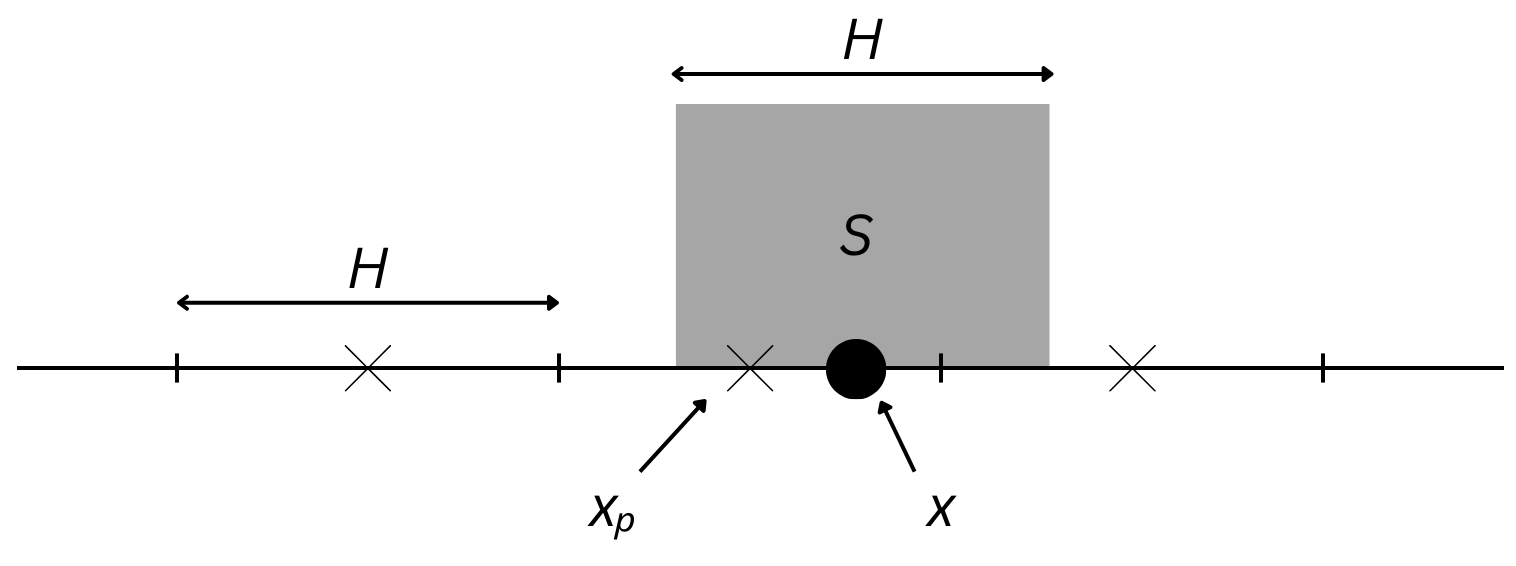
\includegraphics[scale=0.2]{chapters/pm-method/img/CIC.png}
    \caption{The CIC shape centered at $x$ (particle position).
        The particle is within cell $x_p$; however, the cell $x_{p+1}$ gets a non-zero density contribution from the particle.}
    \label{fig:cic-shape}
\end{figure}

In the one-dimensional case, the fraction of mass $W_p$ assigned to mesh-point $p$ from particle at position $x$ is given by
\begin{equation*}
    W(x-x_p) = W_p(x) = \int_{x_p-H/2}^{x_p+H/2} dx' S(x'-x).
\end{equation*}
A simple rule for relating the assignment function $W$ defined above with shape $S$ can be found by noticing that
\begin{equation*}
    W(x) = \int_{-H/2}^{H/2}dx' S(x'-x) = \int_{-\infty}^\infty dx' \Pi\left(\frac{x'}{H}\right)S(x'-x) = \Pi\left(\frac{x}{H}\right) * S(x).
\end{equation*}
This implies that
\begin{align}\label{eq:assignment-functions}
    W_\text{NGP}(x) & = \Pi\left(\frac{x}{H}\right), & W_\text{CIC}(x) & = \Lambda\left(\frac{x}{H}\right), & W_\text{TSC}(x) & = \Pi\left(\frac{x}{H}\right) * \frac{1}{H} \Lambda\left(\frac{x}{H}\right) = (\Pi * \Lambda)\left(\frac{x}{H}\right).
\end{align}
Splitting the domain of integration in the expression for $W_\text{TSC}$ into five disjoint intervals shows that
\begin{equation*}
    (\Pi * \Lambda)(x) = \begin{cases}
        \frac{1}{8}(3-2|x|)^2, & \frac{1}{2} \leq |x| < \frac{3}{2} \\
        \frac{3}{4}-x^2,       & |x| < \frac{1}{2}                  \\
        0,                     & \text{otherwise}.
    \end{cases}
\end{equation*}

Two- and three-dimensional versions of the assignment functions in \autoref{eq:assignment-functions} are products of the assignment functions in each dimension.
For example, the three-dimensional assignment function $W$ is
\begin{equation*}
    W(\mathbf{x}) = W(x)W(y)W(z).
\end{equation*}
Hence, the mass assigned at mesh-point at $\mathbf{x}_\mathbf{p}$ is
\begin{equation*}
    m(\mathbf{x}_\mathbf{p}) = \sum_i m_i W_\mathbf{p}(\mathbf{x}_i),
\end{equation*}
or, in terms of density $\rho$,
\begin{equation}\label{eq:density-assignment}
    \rho(\mathbf{x}_\mathbf{p}) = \frac{1}{V} \sum_i m_i W_\mathbf{p}(\mathbf{x}_i),
\end{equation}
where $V = H^3$ is the volume of a cell and $i$ indexes the particles.

\autoref{eq:density-assignment} is not suitable for direct application in the actual algorithm as it results in $O(N N_g^3)$ time complexity, where $N_g$ is the number of grid points in one dimension.
Instead, we iterate over all particles, identify the parent cell $\mathbf{p}$ of each particle (and the neighborhood of $\mathbf{p}$) and update $\rho$.
This process is illustrated in \autoref{alg:density-assignment}.
\begin{algorithm}
    \caption{Density assignment algorithm}\label{alg:density-assignment}
    \begin{algorithmic}[1]
        \ForAll {particle $i$}
        \ForAll {cell $\mathbf{q}$ in $\mathcal{C}_S(\mathbf{x}_i)$}
        \State $\rho(\mathbf{x}_\mathbf{q}) \gets \rho(\mathbf{x}_\mathbf{q}) + m_i W(\mathbf{x}_i - \mathbf{x}_\mathbf{q}) / V$
        \EndFor
        \EndFor
    \end{algorithmic}
\end{algorithm}
The set $\mathcal{C}_S(\mathbf{x}_i)$ of cells that have to be considered while assigning density from the $i$-th particle depends on the shape $S$ of the particle.
Specifically, we have $\mathcal{C}_\mathrm{NGP}(\mathbf{x}) = \{[\mathbf{x} / H]\}$, $\mathcal{C}_\mathrm{CIC}(\mathbf{x}) = \{\lfloor \mathbf{x}/H \rfloor + \mathbf{t} \;|\; t_i =0,1\}$, and $\mathcal{C}_\mathrm{TSC}(\mathbf{x}) = \{[\mathbf{x} / H] + \mathbf{t} \;|\; t_i = -1, 0, 1\}$.
It follows that $|\mathcal{C}_\mathrm{NGP}(\mathbf{x})| = 1$, $|\mathcal{C}_\mathrm{CIC}(\mathbf{x})| = 8$, and $|\mathcal{C}_\mathrm{TSC}(\mathbf{x})| = 27$ which illustrates the increasing computational cost resulting from using higher-order assignment schemes.
We note that \autoref{alg:density-assignment} is easily parallelized if atomic increments are used in line 3.
